\chapter{Hierarchical Deterministic Wallet} % Main chapter title

\label{hd wallet}
The Hierarchical Deterministic Wallet is defined by BIP32, \textit{bitcoin improvement proposal} number 32 [\cite{1}] and in this chapter we will see in detail how it works.

\section{Elements}
First, let us focus on the main elements of the Wallet:
\begin{itemize}[label=$\diamond$]
	\item Seed.
	\item Extended keys.
\end{itemize}

\subsection{Seed}
The entire Wallet is based on a \textit{seed}.
\\ \\
It is a number taken from a \textit{Discrete Uniform Random Variable}
\begin{equation*}
seed=X(\omega), \qquad X\sim \mathcal{U}(S),
\end{equation*}
where $S$ is the finite set of natural numbers in the range from $1$ to an arbitrary value.\\ Obviously the greater the set from which the number can be extracted, the better it is for the security of the seed itself.
\\ \\
This is an example of seed expressed in hexadecimal format: \\
\textit{seed}=fffcf9f6f3f0edeae7e4e1dedbd8d5d2cfccc9c6c3c0bdbab7b4b1aeaba8a5a29f9c999 \\ 693908d8a8784817e7b7875726f6c696663605d5a5754514e4b484542 

\subsection{Extended Key}
An Extended Key is a sequence of bytes, encoded in base 58. It contains all the information necessary to derive the keys. When the derivation is made for the first time from the seed, the extended key is called master key.
\\ \\
Once it is decoded we will obtain exactly 78 bytes, with a specific meaning and order:
\begin{itemize}[label=$\circledast$]
	\item 4 bytes are used to specified the \textbf{version}.
	\item 1 byte is used to specified the \textbf{depth} in the hierarchical tree: the (master) extended key derived directly from the seed has $depth=0$, its first children have $depth=1$, grandchildren have $depth=2$ and so on.
	\item 4 bytes are used for the \textbf{fingerprint}. It is a unique value that identify the parent. Compute the HASH160 function on the "parent" public key in a compressed form and then take the first 4 bytes:
	\begin{equation*}
	fingerprint=HASH160(\text{parent public key})[0:4],
	\end{equation*}
	where $[0:4]$ is a Python notation.\\
	For the master key the fingerprint is formed by 4 zeros bytes: $fingerprint=0000000000$.
	\item 4 bytes are used to specified the \textbf{index} of the child. \\
	For the master key the index is formed by 4 zeros bytes: $index=0000000000$.
	\item 32 bytes are used for the \textbf{chain code}. The chain code is used in order to introduce entropy in the children generation. We will see below how it works.
	\item 33 bytes are used for the \textbf{key}. It can be \textit{private} or \textit{public}. \\ The public key is expressed in compress form, so the first byte is always $02$ or $03$. The first byte of the private key is always $00$ in order to distinguish it from the public one.\\
\end{itemize}
An extended key is called \textbf{Extended Private Key} if the lasts 33 bytes are used to specify the private key; it is called \textbf{Extended Public Key} if they are used to specify the public key.
\\ \\
For the Bitcoin mainnet it is used for the \textbf{version}: 
\begin{itemize}
	\item $0x0488ADE4$ for an extended private key,
	\item $0x0488B21E$ for an extended public key.
\end{itemize}
When this bytes are encoded in base 58, they returns \textit{xprv} and \textit{xpub} respectively.

\begin{remark}
	Obviously it is possible to calculate the extended public key starting from the extended private key, but it is infeasible to do the opposite. The only difference between the two extended keys are the \textbf{key bytes} and the \textbf{version bytes}, all the others elements remain the same.
\end{remark}

\section{From SEED to Master Private Key}
In this section we will see in detail how it is possible to obtain a \textit{master private key} starting from a \textit{seed}.
\\ \\
First of all we need to convert the seed into a string of bytes, where the most significant bytes come first (big endian). In order to do so, we need to know the length of the string of bytes. \\ \\
Let's see a practical example:
\begin{equation*}
\begin{split}
&byte\_string_1=00\; 00\; 00 \; 07, \\
&byte\_string_2=00\; 00\; 07, \\
&byte\_string_3=00\; 07, \\
&byte\_string_4=07.
\end{split}
\end{equation*}
These $4$ byte strings are obtained from the same seed: $seed=7$ and the only difference is the length of the string.
\begin{remark}
	Different length of the string produces a different master private key, even if the seed is the same number.
\end{remark}
In Python:
\begin{lstlisting}[language=Python]
byte_string = seed.to_bytes(seed_bytes, 'big')
\end{lstlisting}
where $seed$ is an integer number, \textit{seed\_bytes} is the number of bytes that the \textit{byte\_string} should have. 
\\ \\
It is essential to specify the length of the byte string, otherwise, there will be obtained different wallets. 
\\ \\
Once we obtain a string of bytes, we will compute the HMAC algorithm. The hash function used for HMAC is the SHA512 and the \textit{key} is a particular string of bytes: \textit{b"Bitcoin seed"}. In Python the implementation is the following:

\begin{lstlisting}[language=Python]
from hashlib import sha512
from hmac import HMAC

hashValue = HMAC(b"Bitcoin seed", byte_string, sha512).digest()
\end{lstlisting}
where \textit{.digest()} is used in order to return a string of bytes.
\\ \\
Now we have obtained a \textit{hashValue} of $512$ bits, so $64$ bytes. Consider the firsts $32$ bytes as the master private key and the next $32$ bytes as the master chain code. A Python implementation is the following:

\begin{lstlisting}[language=Python]
private_key_bytes = hashValue[0:32]
chain_code_bytes = hashValue[32:64]
\end{lstlisting}
\begin{flushleft}
	Now we have two-byte strings, one for the master private key and the other for the master chain code.
\end{flushleft}
It is important to remember that a private key must be in the range between $1$ and $order$, so the byte string for the private key should be converted in \textit{int} and then take the \textit{mod order}. In Python we have:

\begin{lstlisting}[language=Python]
private_key = int(private_key_bytes.hex(), 16) % order
\end{lstlisting}
\begin{flushleft}
	Finally, we will concatenate all the information obtained in order to form a Master Extended Private Key (in bytes format):
\end{flushleft}

\begin{itemize}
	\item vbytes = $b'\backslash x04\backslash x88\backslash xAD\backslash xE4'$,
	\item depth = $b'\backslash x00'$,
	\item fingerprint = $b'\backslash x00\backslash x00\backslash x00\backslash x00'$,
	\item index = $b'\backslash x00\backslash x00\backslash x00\backslash x00'$,
	\item chain code is the one previously computed,
	\item private key = $b'\backslash x00'$ $+$ private key in bytes format, previously computed.
\end{itemize}
Then the Master Extended Private Key is formed by concatenation:

\begin{lstlisting}[language=Python]
xkey = vbytes + depth + fingerprint + index + chain_code + key
\end{lstlisting}
\begin{flushleft}
	In order to make it readable, a base58 encoding is performed.
\end{flushleft}
This is an example of Master Extended Private Key: \\
xprv9s21ZrQH143K3wEaiSJZ8jYCuZF1oJoXHiwFcx2WwXqQHD4ZLdyEAFZ22M4 BmQT82HRbWssLArj53YDQTj6vSN4iH6nTiSQ61C5CckxUtDq.

\begin{remark}
	The SHA512 is an irreversible function, so it is infeasible to obtain the seed, knowing the master key. (It is also useless because with the master key you can derive all the keys in the wallet).
\end{remark}

\begin{flushleft}
	Graphically these operations can be shown in Figure \ref{fig:From seed to master private key}.
\end{flushleft}

\begin{figure}[ht!]
	\centering
	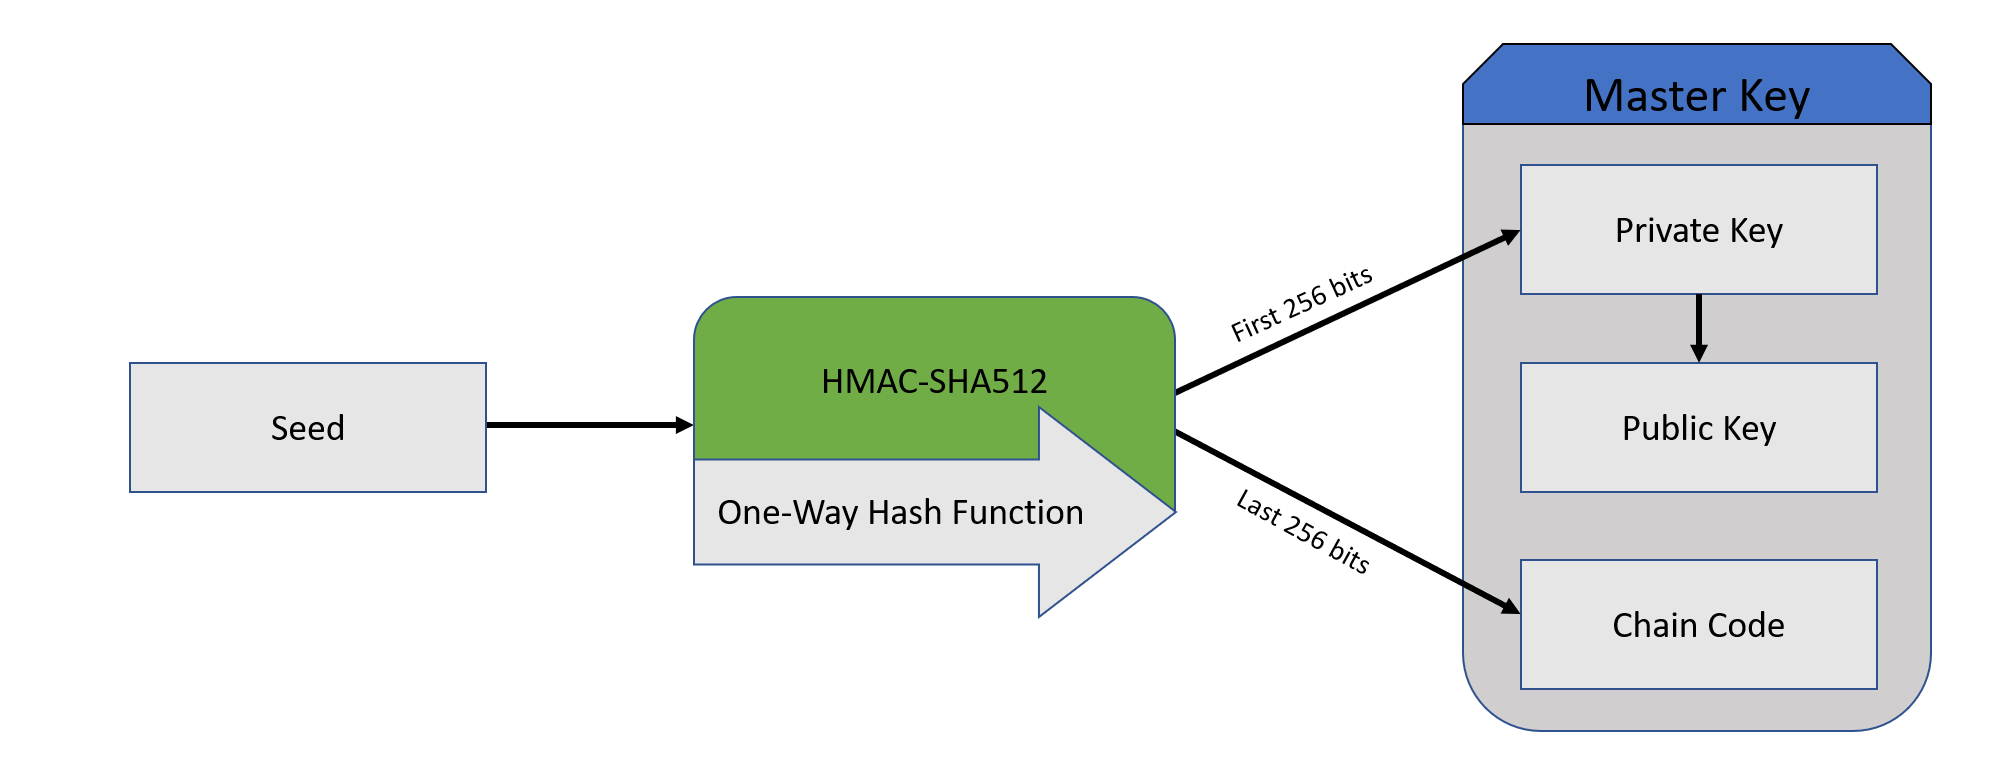
\includegraphics[width=14.5cm]{Figures/seed_to_xprv_v2.png}
	\caption{From seed to master private key}
	\label{fig:From seed to master private key}
\end{figure}


\section{Child Key derivation}
In this section, we will see how it is possible to derive different child key from a single extended private key. There are two methods:
\begin{itemize}
	\item Normal.
	\item Hardened.
\end{itemize}
Both methods have some advantage and disadvantage that we will discuss later. For every situation, it is essential to use the method that best fit.
\\ \\
For both the method the derivation starts from an extended private key. From this key some essential information are necessary:
\begin{itemize}[label=$\star$]
	\item Chain code.
	\item Private key.
\end{itemize}
It is also required a number, used in order to specify the \textbf{index} of the child. This number should be in the range between $0$ and $4294967295$. This is due to the fact that in any extended key there are 4 bytes used to specify the index of the child:
\begin{equation*}
max \; index=(FF\;FF\;FF\;FF)_{base \; 16} = 2^{32}-1 = 4294967295.
\end{equation*}
In fact, it is possible to generate even a greater number of children from the same parent, but it would not be possible to write the corresponding extended key in the format described above.


\subsection{Normal derivation}

First, we need to compute the Parent Public Key $P$. This is obtained from the usual scalar multiplication between a point on the EC (the Generator $G$) and the Parent Private Key $p$:
\begin{equation*}
P=p\cdot G.
\end{equation*}
Then we consider only the compress form of $P$ and convert this value into a byte string, obtaining 33 bytes.
\\ \\
After that we concatenate this 33 byte string to the 4 byte string representing the index number:
\begin{equation*}
msg = compressed \; public\;key \;|\; index,
\end{equation*}
where $msg$ is now a string of $37$ bytes. \\ \\
Finally, we apply the HMAC algorithm with the following inputs:

\begin{itemize}[label=$\odot$]
	\item \textbf{Hash function}: SHA512.
	\item \textbf{Key}: chain code.
	\item \textbf{Message}: $msg$.
\end{itemize}
The Python code is the following:
\begin{lstlisting}[language=Python]
from hmac import HMAC
from hashlib import sha512

msg=parent_public_key + index
hashValue = HMAC(parent_chain_code, msg, sha512).digest()
\end{lstlisting}
\begin{flushleft}
	The result is a string of 64 bytes: \textit{hashValue}.
\end{flushleft}
Now we split this string of bytes in two: the last 32 are the child chain code. Then we take the first 32 bytes, convert them into an integer number and sum it to the parent private key (mod \textit{order}), obtaining the child private key.\\ \\
This is the Python code:

\begin{lstlisting}[language=Python]
child_chain_code = hashValue[32:]
q = int(hashValue[:32].hex(), 16)
child_private_key = (q + parent_private_key) % order
\end{lstlisting}

\begin{flushleft}
	Graphically these operations can be shown in Figure \ref{fig:normal_derivation}.
\end{flushleft}

\begin{figure}[ht!]
	\centering
	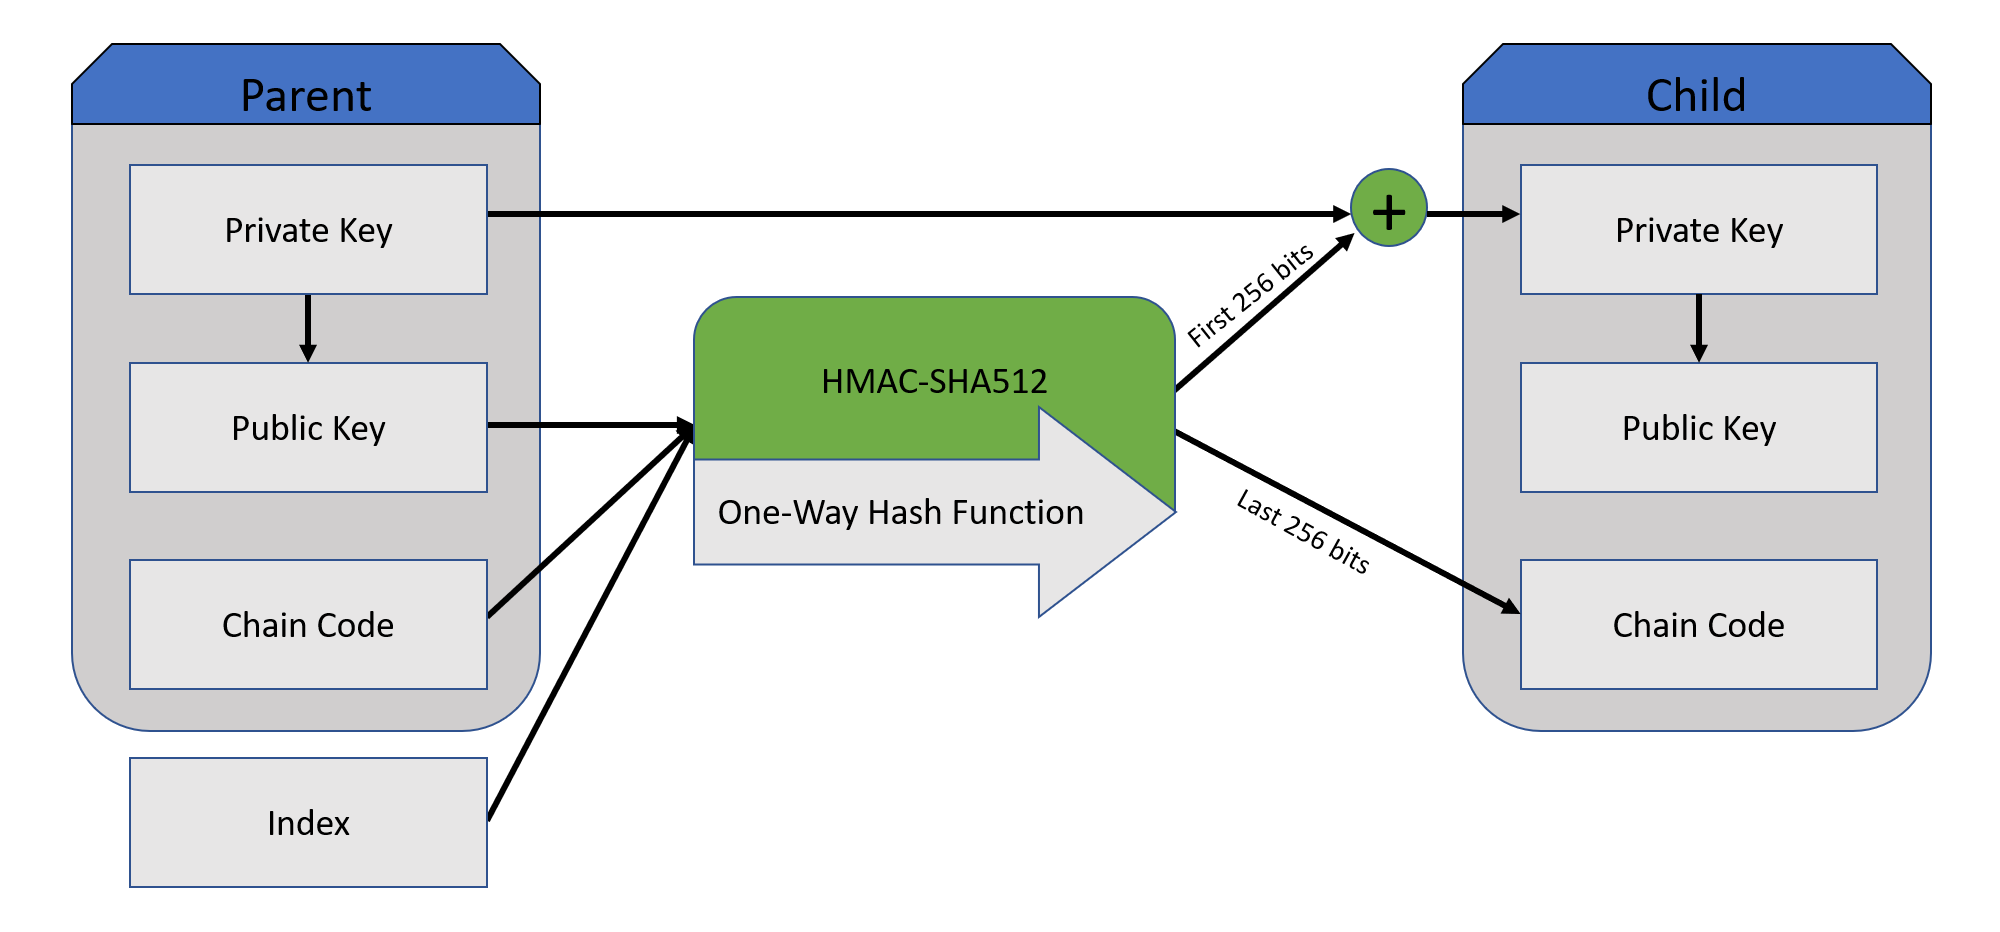
\includegraphics[width=14.5cm]{Figures/normal_derivation_v2.png}
	\caption{Normal Derivation }
	\label{fig:normal_derivation}
\end{figure}


\subsection{Hardened derivation}
This method is similar to the previous one, the only difference is that as input of the \textit{hash} function the private key is used instead of the public one. \\ \\
First, we concatenate the 33 bytes of parent private key, considering also the $00$ byte, with the 4 byte string representing the index number.

\begin{remark}
In order to better distinguish the hardened derivation from the normal one, the numbering of the indices starts from the number $2^{31}.$
\end{remark} 
\begin{equation*}
msg = 00 \;|\; private\;key \;|\; index,
\end{equation*}
where $msg$ is now a string of $37$ bytes. \\ \\
Then we apply the HMAC algorithm with the following inputs:

\begin{itemize}[label=$\odot$]
	\item \textbf{Hash function}: SHA512.
	\item \textbf{Key}: chain code.
	\item \textbf{Message}: $msg$.
\end{itemize}
The Python code is the following:
\begin{lstlisting}[language=Python]
from hmac import HMAC
from hashlib import sha512

msg=parent_private_key + index
hashValue = HMAC(parent_chain_code, msg, sha512).digest()
\end{lstlisting}
\begin{flushleft}
	The result is a string of 64 bytes: \textit{hashValue}. In this code the $parent\_private\_key$ already has the first $00$ byte, because it is taken directly from the parent extended private key.
\end{flushleft}
Now we split this string of bytes in two (in the same way as the normal method): the last 32 are the child chain code. Finally, we take the first 32 bytes, convert them into an integer number and sum it to the parent private key (mod \textit{order}), obtaining the child private key.\\ \\
This is the Python code:

\begin{lstlisting}[language=Python]
child_chain_code = hashValue[32:]
q = int(hashValue[:32].hex(), 16)
child_private_key = (q + parent_private_key) % order
\end{lstlisting}


\begin{flushleft}
	Graphically these operations can be shown in Figure \ref{fig:hardened_derivation}.
\end{flushleft}

\begin{figure}[ht!]
	\centering
	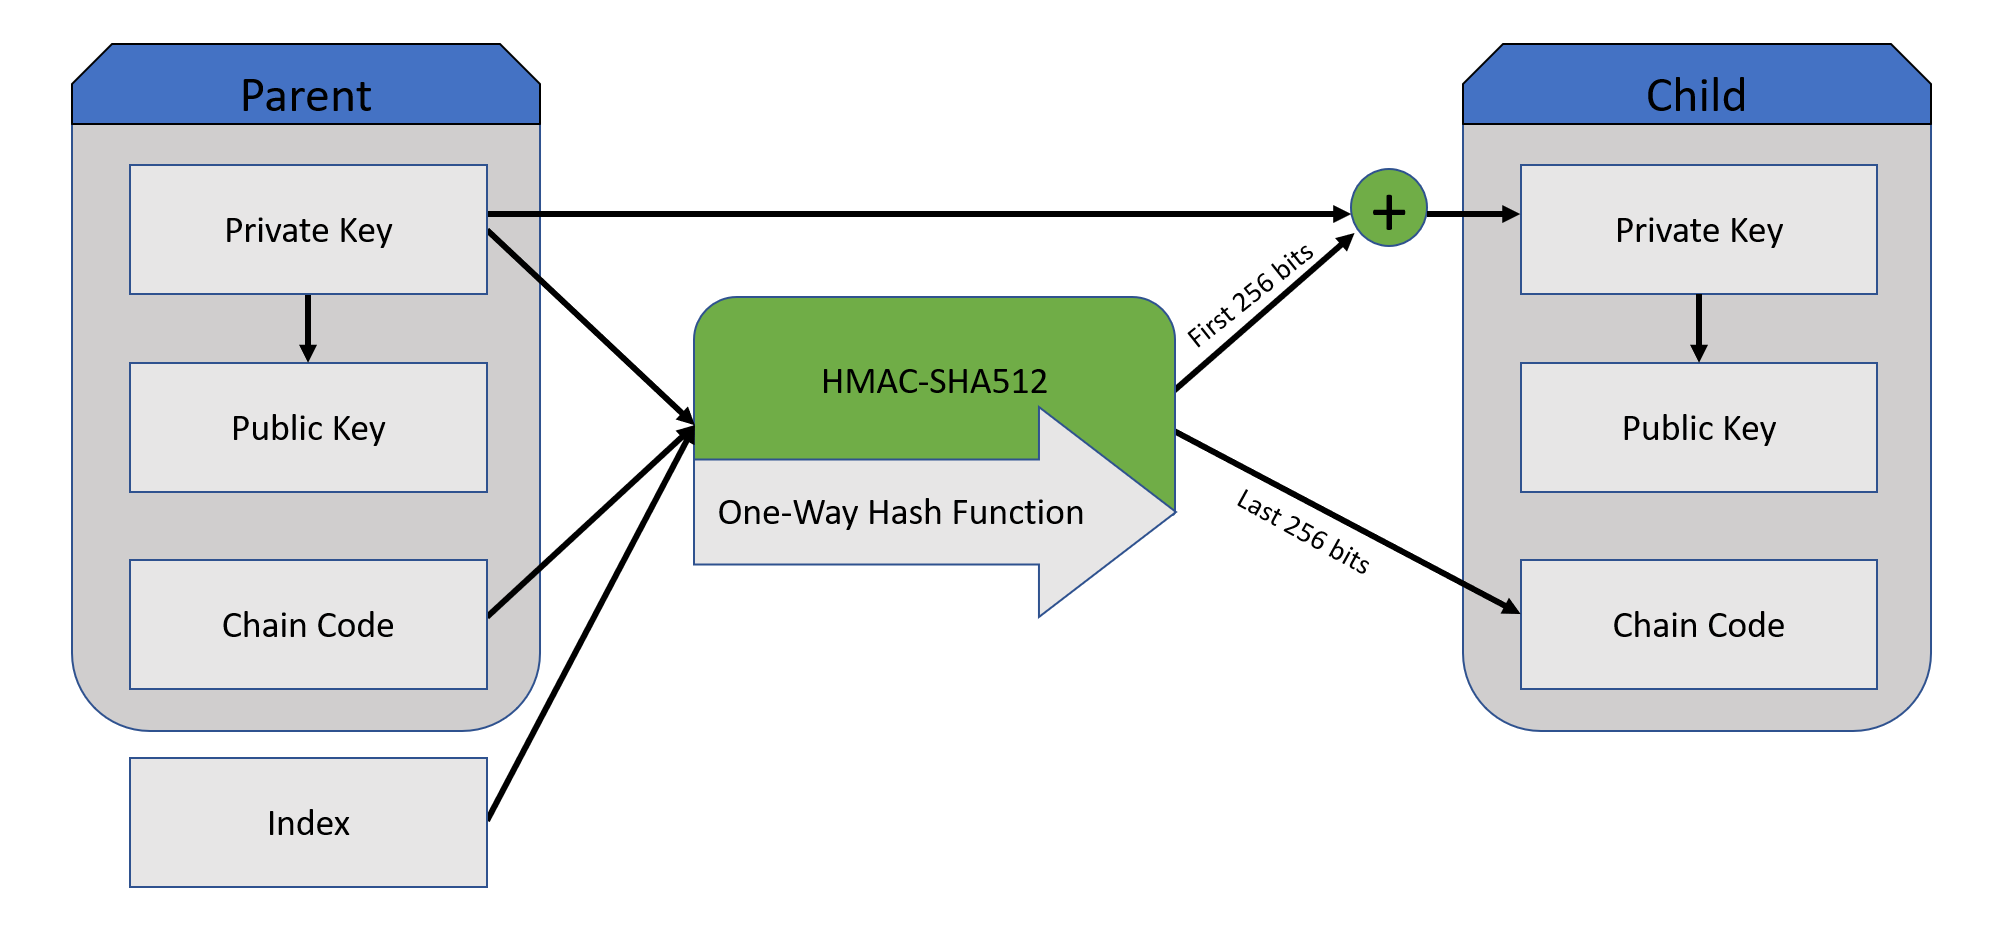
\includegraphics[width=14.5cm]{Figures/hardened_derivation_v2.png}
	\caption{Hardened Derivation }
	\label{fig:hardened_derivation}
\end{figure}


\section{Special derivation}
Using a \textit{normal derivation} it is possible to derive the extended public key, starting only from the extended public key of the parent.

\subsection{Public derivation}

In order to compute this particular derivation, the only essential elements are the ones contained in the extended public key, in particular:

\begin{itemize}
	\item Public key $P_{parent}$.
	\item Chain code.
	\item Index.
\end{itemize}
First, we apply the HMAC algorithm to the same inputs used for the normal derivation:
\begin{itemize}[label=$\odot$]
	\item \textbf{Hash function}: SHA512;
	\item \textbf{Key}: chain code;
	\item \textbf{Message}: $msg$;
\end{itemize}
where $msg$ is obtained as before:
\begin{equation*}
msg = compressed \; public\;key \;|\; index.
\end{equation*}
The output of this function is the same of the normal derivation with the extended private key. The last 32 bytes formed the child chain code, instead, the first 32 bytes can be read as a special number: $q$. 
\\ \\
Now we multiply the generator $G$ to the integer number $q$ and we obtain $Q$, a point on the EC:
\begin{equation*}
Q=q\cdot G.
\end{equation*}
Finally, we compute the sum between two points on the elliptic curve: $Q$ and $P_{parent}$, where $P_{parent}$ is the parent public key.
\begin{equation*}
Q+P_{parent}=P_{child},
\end{equation*}
where $P_{child}$ is the child public key. 
\\ \\
We will now prove that the child public key obtained in this way $P_{child_2}$ is the same as that obtained starting from the private key, $P_{child_1}$:
\\ \\
Both the procedures start from $q$, number obtained from the first 32 bytes of the HMAC function. Let's call $p_{parent}$ the parent private key and $p_{child}$ the child private key.

\begin{equation*} \label{eq2}
\begin{split}
P_{child_1} & = p_{child} \cdot G \\
& = (q+p_{parent}) \cdot G \\
& = (q \cdot G) + (p_{parent}\cdot G) \\
& = Q + P_{parent} = P_{child_2}
\end{split}
\end{equation*}
\begin{flushright}
	\textit{cvd}
\end{flushright}
Graphically this derivation can be shown in Figure \ref{fig:pubtopub}.
\begin{figure}[ht!]
	\centering
	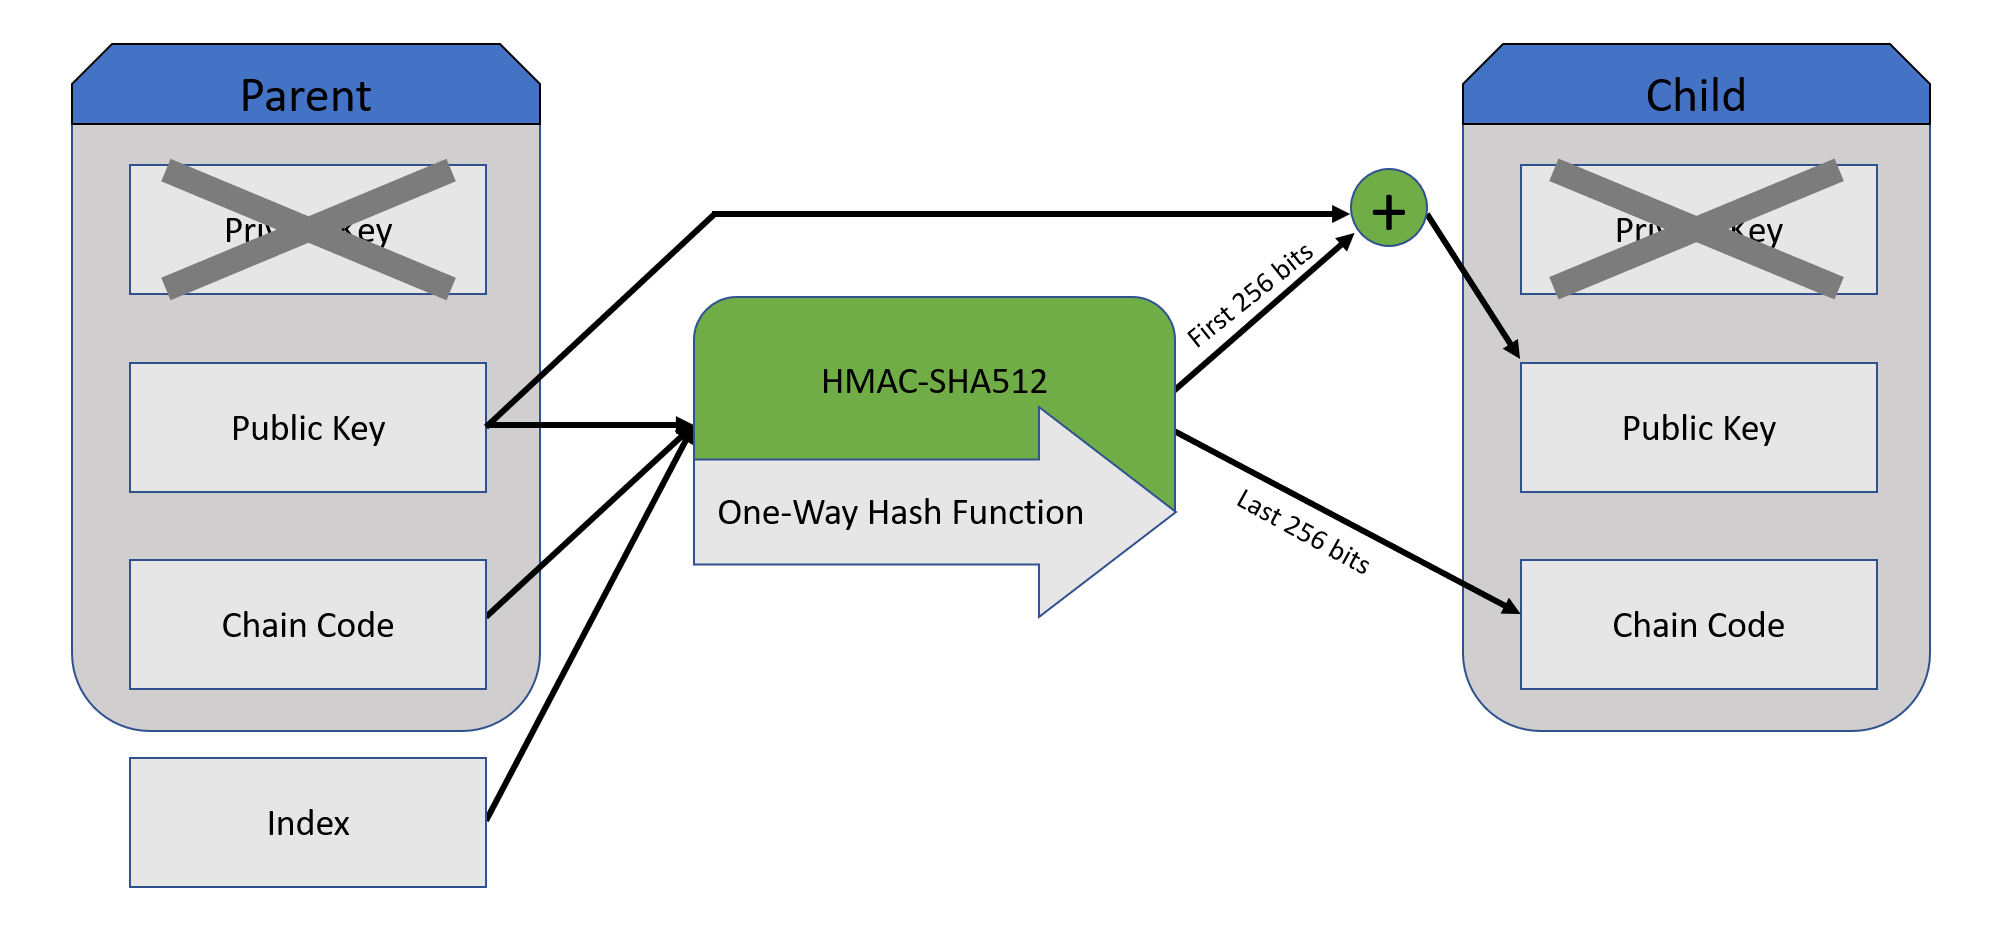
\includegraphics[width=14.5cm]{Figures/pubtopub.png} %cambiare immagine
	\caption{Public Derivation}
	\label{fig:pubtopub}
\end{figure}

\subsection{Weakness of Normal Derivation}
As shown above, the normal derivation presents a great advantage, but also a weakness. It is possible to derive the \textbf{parent extended private key} knowing the \textbf{parent extended public key} and only one of the \textbf{child extended private key}.
\\ \\
The HMAC-SHA256 function has as inputs three elements: the parent chain code, the parent public key and the child index. The firsts two information can be taken from the parent extended public key, instead the child index can be taken from the child extended private key.

\begin{equation*}
msg = compressed \;parent\; public\;key \;|\;child\; index.
\end{equation*}
Now we apply the HMAC algorithm with the usual inputs:

\begin{itemize}[label=$\odot$]
	\item \textbf{Hash function}: SHA512.
	\item \textbf{Key}: parent chain code.
	\item \textbf{Message}: $msg$.
\end{itemize}
After that, we consider the first 32 bytes of the result of this function and consider it as an integer number, $q$.
\\ \\
Remembering that to get the child private key it is needed to compute a sum with the parent private key, it is possible to reverse the process. \\ \\
Let's call $p_{child}$ and $p_{parent}$ the private keys of the child and the parent respectively.
\begin{equation}\label{eq3}
\begin{split}
p_{child} &= q+p_{parent} \qquad \mod (order) \\
&\Downarrow \\
p_{parent} &=p_{child}-q \qquad \mod (order)
\end{split}
\end{equation}
The implication (\ref{eq3}) holds also with modular arithmetic.
\\ \\
So we have derived the private key of the parent. Graphically this derivation can be shown in Figure \ref{fig:from_child_to_parent}
\begin{figure}[ht!]
	\centering
	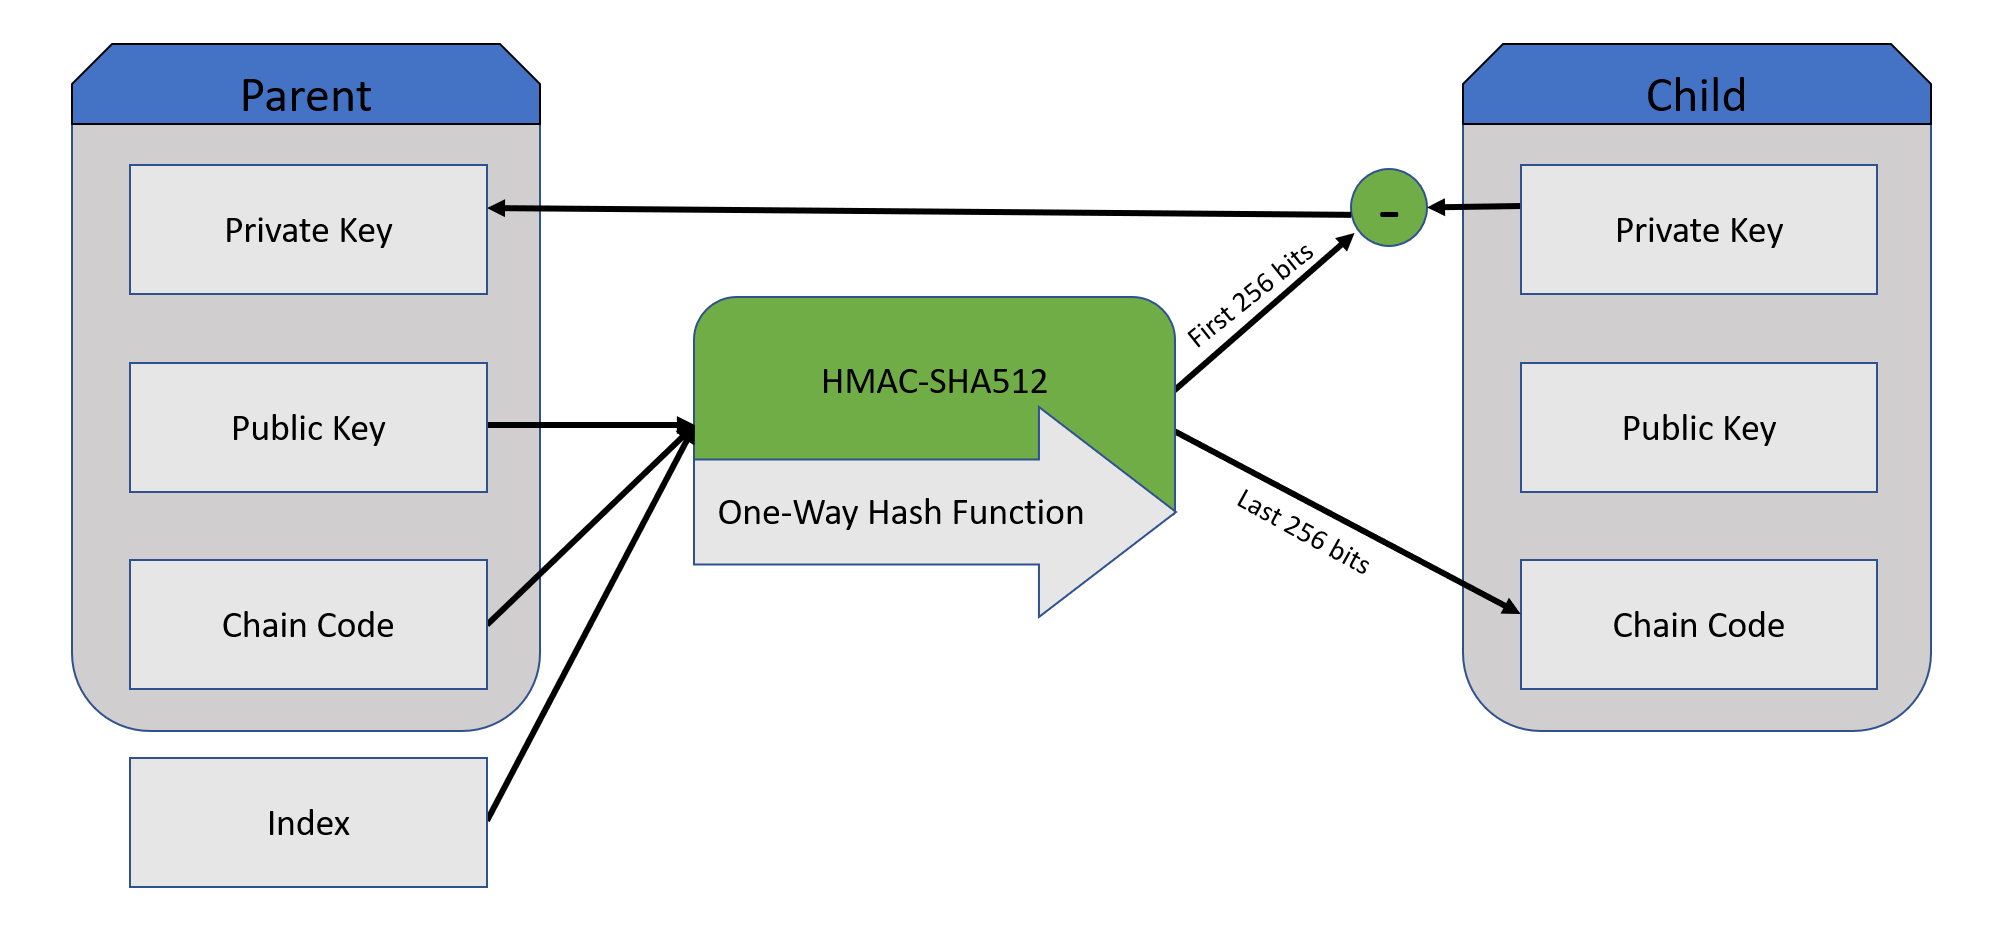
\includegraphics[width=14.5cm]{Figures/childtoparent.png} %cambiare immagine
	\caption{From child to parent}
	\label{fig:from_child_to_parent}
\end{figure}



\section{Advantages and disadvantages}
We have seen that public-to-public operation is possible using the normal derivation. This is impossible with the hardened one.
\\ \\
In fact, the inputs of HMAC-SHA512 are different for the two derivations. If for the normal derivation only the information in the public extended key is sufficient, for the hardened derivation the parent private key is needed. This makes impossible to obtain a public from a public, but also it makes impossible to derive the private key of the parent knowing the private key of the child and the public of the parent.
\\ \\
It is advisable to use each of the two methods in the appropriate situations.

\subsection{When to use Normal Derivation?}
Normal derivation should be used whenever all the child keys are collected in the same digital place and you should never give one key to someone else. As already mentioned a leak of a single private key can compromise the entire wallet.
\\ \\
However, if all the child keys are used by the same person and you need to generate a different public key, with this derivation it is possible to do so even in a "hot place". Let's suppose to have stored only the extended public key in a device, you can then receive payment to your public keys, but it is impossible to spend those coins as long as the private keys are hidden. If someone stole your device the only problem is a leak of privacy, because it is possible, by examining the blockchain, to discover all transactions signed with the private keys associated with the public keys of the wallet, but it is impossible to sign new transactions without having the private keys.


\subsection{When to use Hardened Derivation?}
Hardened derivation should be used whenever all the keys generated are used for different purposes or are stored in different places. With this procedure, it is possible to yield a branch of the tree to someone else in order to manage part of your money, without the risk to lose all the others keys in the wallet.
\\ \\
As a best practice, it is always advisable to use the hardened method for the first derivation from the extended master private key. A hardened key should have both hardened or normal children, but from a normal child, it is not reasonable to derive a hardened one because it makes no sense to increase the security of the wallet at the last level.


